\documentclass[]{article}
\usepackage{lmodern}
\usepackage{amssymb,amsmath}
\usepackage{ifxetex,ifluatex}
\usepackage{fixltx2e} % provides \textsubscript
\ifnum 0\ifxetex 1\fi\ifluatex 1\fi=0 % if pdftex
  \usepackage[T1]{fontenc}
  \usepackage[utf8]{inputenc}
\else % if luatex or xelatex
  \ifxetex
    \usepackage{mathspec}
  \else
    \usepackage{fontspec}
  \fi
  \defaultfontfeatures{Ligatures=TeX,Scale=MatchLowercase}
\fi
% use upquote if available, for straight quotes in verbatim environments
\IfFileExists{upquote.sty}{\usepackage{upquote}}{}
% use microtype if available
\IfFileExists{microtype.sty}{%
\usepackage{microtype}
\UseMicrotypeSet[protrusion]{basicmath} % disable protrusion for tt fonts
}{}
\usepackage[margin=1in]{geometry}
\usepackage{hyperref}
\hypersetup{unicode=true,
            pdftitle={Replication Code},
            pdfborder={0 0 0},
            breaklinks=true}
\urlstyle{same}  % don't use monospace font for urls
\usepackage{color}
\usepackage{fancyvrb}
\newcommand{\VerbBar}{|}
\newcommand{\VERB}{\Verb[commandchars=\\\{\}]}
\DefineVerbatimEnvironment{Highlighting}{Verbatim}{commandchars=\\\{\}}
% Add ',fontsize=\small' for more characters per line
\usepackage{framed}
\definecolor{shadecolor}{RGB}{248,248,248}
\newenvironment{Shaded}{\begin{snugshade}}{\end{snugshade}}
\newcommand{\AlertTok}[1]{\textcolor[rgb]{0.94,0.16,0.16}{#1}}
\newcommand{\AnnotationTok}[1]{\textcolor[rgb]{0.56,0.35,0.01}{\textbf{\textit{#1}}}}
\newcommand{\AttributeTok}[1]{\textcolor[rgb]{0.77,0.63,0.00}{#1}}
\newcommand{\BaseNTok}[1]{\textcolor[rgb]{0.00,0.00,0.81}{#1}}
\newcommand{\BuiltInTok}[1]{#1}
\newcommand{\CharTok}[1]{\textcolor[rgb]{0.31,0.60,0.02}{#1}}
\newcommand{\CommentTok}[1]{\textcolor[rgb]{0.56,0.35,0.01}{\textit{#1}}}
\newcommand{\CommentVarTok}[1]{\textcolor[rgb]{0.56,0.35,0.01}{\textbf{\textit{#1}}}}
\newcommand{\ConstantTok}[1]{\textcolor[rgb]{0.00,0.00,0.00}{#1}}
\newcommand{\ControlFlowTok}[1]{\textcolor[rgb]{0.13,0.29,0.53}{\textbf{#1}}}
\newcommand{\DataTypeTok}[1]{\textcolor[rgb]{0.13,0.29,0.53}{#1}}
\newcommand{\DecValTok}[1]{\textcolor[rgb]{0.00,0.00,0.81}{#1}}
\newcommand{\DocumentationTok}[1]{\textcolor[rgb]{0.56,0.35,0.01}{\textbf{\textit{#1}}}}
\newcommand{\ErrorTok}[1]{\textcolor[rgb]{0.64,0.00,0.00}{\textbf{#1}}}
\newcommand{\ExtensionTok}[1]{#1}
\newcommand{\FloatTok}[1]{\textcolor[rgb]{0.00,0.00,0.81}{#1}}
\newcommand{\FunctionTok}[1]{\textcolor[rgb]{0.00,0.00,0.00}{#1}}
\newcommand{\ImportTok}[1]{#1}
\newcommand{\InformationTok}[1]{\textcolor[rgb]{0.56,0.35,0.01}{\textbf{\textit{#1}}}}
\newcommand{\KeywordTok}[1]{\textcolor[rgb]{0.13,0.29,0.53}{\textbf{#1}}}
\newcommand{\NormalTok}[1]{#1}
\newcommand{\OperatorTok}[1]{\textcolor[rgb]{0.81,0.36,0.00}{\textbf{#1}}}
\newcommand{\OtherTok}[1]{\textcolor[rgb]{0.56,0.35,0.01}{#1}}
\newcommand{\PreprocessorTok}[1]{\textcolor[rgb]{0.56,0.35,0.01}{\textit{#1}}}
\newcommand{\RegionMarkerTok}[1]{#1}
\newcommand{\SpecialCharTok}[1]{\textcolor[rgb]{0.00,0.00,0.00}{#1}}
\newcommand{\SpecialStringTok}[1]{\textcolor[rgb]{0.31,0.60,0.02}{#1}}
\newcommand{\StringTok}[1]{\textcolor[rgb]{0.31,0.60,0.02}{#1}}
\newcommand{\VariableTok}[1]{\textcolor[rgb]{0.00,0.00,0.00}{#1}}
\newcommand{\VerbatimStringTok}[1]{\textcolor[rgb]{0.31,0.60,0.02}{#1}}
\newcommand{\WarningTok}[1]{\textcolor[rgb]{0.56,0.35,0.01}{\textbf{\textit{#1}}}}
\usepackage{graphicx,grffile}
\makeatletter
\def\maxwidth{\ifdim\Gin@nat@width>\linewidth\linewidth\else\Gin@nat@width\fi}
\def\maxheight{\ifdim\Gin@nat@height>\textheight\textheight\else\Gin@nat@height\fi}
\makeatother
% Scale images if necessary, so that they will not overflow the page
% margins by default, and it is still possible to overwrite the defaults
% using explicit options in \includegraphics[width, height, ...]{}
\setkeys{Gin}{width=\maxwidth,height=\maxheight,keepaspectratio}
\IfFileExists{parskip.sty}{%
\usepackage{parskip}
}{% else
\setlength{\parindent}{0pt}
\setlength{\parskip}{6pt plus 2pt minus 1pt}
}
\setlength{\emergencystretch}{3em}  % prevent overfull lines
\providecommand{\tightlist}{%
  \setlength{\itemsep}{0pt}\setlength{\parskip}{0pt}}
\setcounter{secnumdepth}{0}
% Redefines (sub)paragraphs to behave more like sections
\ifx\paragraph\undefined\else
\let\oldparagraph\paragraph
\renewcommand{\paragraph}[1]{\oldparagraph{#1}\mbox{}}
\fi
\ifx\subparagraph\undefined\else
\let\oldsubparagraph\subparagraph
\renewcommand{\subparagraph}[1]{\oldsubparagraph{#1}\mbox{}}
\fi

%%% Use protect on footnotes to avoid problems with footnotes in titles
\let\rmarkdownfootnote\footnote%
\def\footnote{\protect\rmarkdownfootnote}

%%% Change title format to be more compact
\usepackage{titling}

% Create subtitle command for use in maketitle
\providecommand{\subtitle}[1]{
  \posttitle{
    \begin{center}\large#1\end{center}
    }
}

\setlength{\droptitle}{-2em}

  \title{Replication Code}
    \pretitle{\vspace{\droptitle}\centering\huge}
  \posttitle{\par}
    \author{}
    \preauthor{}\postauthor{}
    \date{}
    \predate{}\postdate{}
  

\begin{document}
\maketitle

\hypertarget{usage-of-package-sammcmc}{%
\section{\texorpdfstring{Usage of package
\textbf{samMCMC}}{Usage of package samMCMC}}\label{usage-of-package-sammcmc}}

Suppose we want to sample from a simple normal distribution. This of
course can most easily and efficiently be done with the \texttt{rnorm}
function in the core \textbf{stats} package; however, to demonstrate the
usage of \textbf{samMCMC} we can start with this simple case. To sample
from a normal distribution we first define its density

\begin{Shaded}
\begin{Highlighting}[]
\CommentTok{# normal density where `x` is the variable, the first element of `pars` is the mean}
\CommentTok{# and the second element of `pars` is the S.D.}
\NormalTok{egFunc <-}\StringTok{ }\ControlFlowTok{function}\NormalTok{(x, pars) \{}
    \KeywordTok{dnorm}\NormalTok{(x, pars[}\DecValTok{1}\NormalTok{], pars[}\DecValTok{2}\NormalTok{])}
\NormalTok{\}}
\end{Highlighting}
\end{Shaded}

Now we can use of \texttt{samMCMC} to sample from, in this example, a
normal \(N(1, 4)\) distribution.

\begin{Shaded}
\begin{Highlighting}[]
\CommentTok{# control parameters for `samMCMC`}
\NormalTok{numSampBurn <-}\StringTok{ }\DecValTok{100}
\NormalTok{t0 <-}\StringTok{ }\DecValTok{100}
\NormalTok{numSamp <-}\StringTok{ }\DecValTok{1000}
\NormalTok{numSampBurn <-}\StringTok{ }\DecValTok{10000}
\NormalTok{thinning <-}\StringTok{ }\DecValTok{100}

\CommentTok{# sample; we set control parameters `direct` to `TRUE` because we are directly}
\CommentTok{# sampling from the density}
\NormalTok{xsamp <-}\StringTok{ }\KeywordTok{samMCMC}\NormalTok{(egFunc, }\DataTypeTok{init =} \DecValTok{0}\NormalTok{, }\DataTypeTok{pars =} \KeywordTok{c}\NormalTok{(}\DecValTok{1}\NormalTok{, }\DecValTok{2}\NormalTok{), }
               \DataTypeTok{control =} \KeywordTok{list}\NormalTok{(}\DataTypeTok{numSamp =}\NormalTok{ numSamp, }\DataTypeTok{t0 =}\NormalTok{ t0, }\DataTypeTok{numSampBurn =}\NormalTok{ numSampBurn,}
                              \DataTypeTok{thinning =}\NormalTok{ thinning, }\DataTypeTok{direct =} \OtherTok{TRUE}\NormalTok{))}
\end{Highlighting}
\end{Shaded}

We can then compare the sample from \texttt{samMCMC} to its known
generative distribution visually

\begin{Shaded}
\begin{Highlighting}[]
\KeywordTok{plot}\NormalTok{(}\KeywordTok{ecdf}\NormalTok{(xsamp}\OperatorTok{$}\NormalTok{X_mat[}\DecValTok{1}\NormalTok{, ]), }\DataTypeTok{lwd =} \DecValTok{3}\NormalTok{)}
\KeywordTok{curve}\NormalTok{(}\KeywordTok{pnorm}\NormalTok{(x, }\DecValTok{1}\NormalTok{, }\DecValTok{2}\NormalTok{), }\DataTypeTok{add =} \OtherTok{TRUE}\NormalTok{, }\DataTypeTok{col =} \StringTok{'red'}\NormalTok{)}
\end{Highlighting}
\end{Shaded}

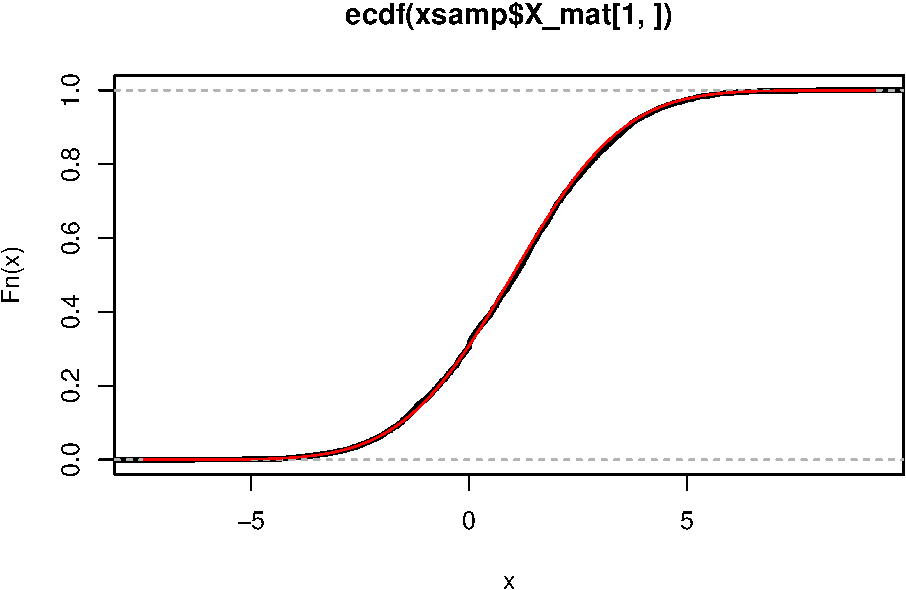
\includegraphics{replication_code_files/figure-latex/unnamed-chunk-3-1.pdf}

We can also use \texttt{samMCMC} to sample given a cost function as
described earlier. To do this we define a cost function (for simplicity
we again use a normal distribution) and specify
\texttt{direct\ =\ FALSE} in the control parameters in addition to
specifying a temperature.

\begin{Shaded}
\begin{Highlighting}[]
\CommentTok{# normal likelihood where `m` is the mean (sd is fixed at 2) and `dat` are the data}
\NormalTok{egCostFunc <-}\StringTok{ }\ControlFlowTok{function}\NormalTok{(m, dat) \{}
    \OperatorTok{-}\StringTok{ }\KeywordTok{sum}\NormalTok{(}\KeywordTok{dnorm}\NormalTok{(dat, m, }\DecValTok{2}\NormalTok{, }\DataTypeTok{log =} \OtherTok{TRUE}\NormalTok{))}
\NormalTok{\}}

\CommentTok{# example data}
\NormalTok{egData <-}\StringTok{ }\KeywordTok{rnorm}\NormalTok{(}\DecValTok{5000}\NormalTok{, }\DecValTok{1}\NormalTok{, }\DecValTok{2}\NormalTok{)}

\CommentTok{# sample using previously defined control parameters but now with `direct = TRUE` and `temp = 1`}
\NormalTok{xsamp <-}\StringTok{ }\KeywordTok{samMCMC}\NormalTok{(egCostFunc, }\DataTypeTok{init =} \DecValTok{0}\NormalTok{, }\DataTypeTok{dat =}\NormalTok{ egData, }
               \DataTypeTok{control =} \KeywordTok{list}\NormalTok{(}\DataTypeTok{numSamp =}\NormalTok{ numSamp, }\DataTypeTok{t0 =}\NormalTok{ t0, }\DataTypeTok{numSampBurn =}\NormalTok{ numSampBurn,}
                              \DataTypeTok{thinning =}\NormalTok{ thinning, }\DataTypeTok{direct =} \OtherTok{FALSE}\NormalTok{, }\DataTypeTok{temp =} \DecValTok{1}\NormalTok{))}
\end{Highlighting}
\end{Shaded}

Again, we can compare this sample from \texttt{samMCMC} with its known
distribution, in this case the sampling distribution of the MLE for the
mean of a normal distribution with known variance, which is
\(N(\hat{\mu}, \sqrt{\sigma^2 / N})\).

\begin{Shaded}
\begin{Highlighting}[]
\KeywordTok{plot}\NormalTok{(}\KeywordTok{ecdf}\NormalTok{(xsamp}\OperatorTok{$}\NormalTok{X_mat[}\DecValTok{1}\NormalTok{, ]))}
\NormalTok{mleSD <-}\StringTok{ }\KeywordTok{sqrt}\NormalTok{(}\DecValTok{4} \OperatorTok{/}\StringTok{ }\KeywordTok{length}\NormalTok{(egData))}
\KeywordTok{curve}\NormalTok{(}\KeywordTok{pnorm}\NormalTok{(x, }\DataTypeTok{mean =} \DecValTok{1}\NormalTok{, }\DataTypeTok{sd =}\NormalTok{ mleSD), }\DataTypeTok{add =} \OtherTok{TRUE}\NormalTok{, }\DataTypeTok{col =} \StringTok{'red'}\NormalTok{)}
\end{Highlighting}
\end{Shaded}

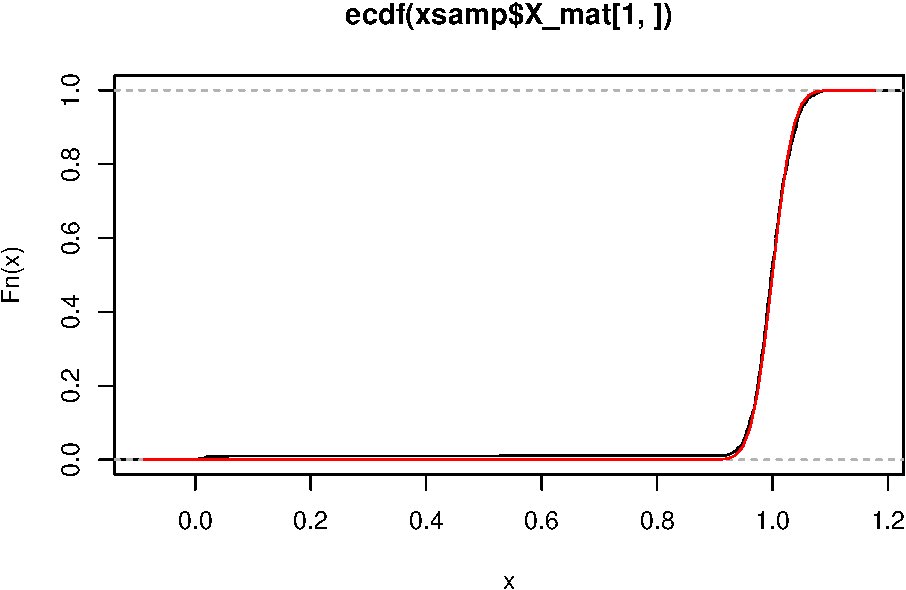
\includegraphics{replication_code_files/figure-latex/unnamed-chunk-5-1.pdf}

A more realistic use case of \texttt{samMCMC} is when the distribution
we would like to sample from cannot be easily inverted, or the
distribution we would like to approximate with a sample cannot be
expressed analytically. We take as a simple example a mixture of normal
distributions. In this example we use an equal mixture of three normals:
\(N(-1, 0.5)\), \(N(0, 1.5)\), \(N(1, 0.75\).

\begin{Shaded}
\begin{Highlighting}[]
\NormalTok{mixFunc <-}\StringTok{ }\ControlFlowTok{function}\NormalTok{(x) \{}
    \DecValTok{1}\OperatorTok{/}\DecValTok{3} \OperatorTok{*}\StringTok{ }\KeywordTok{dnorm}\NormalTok{(x, }\DecValTok{-3}\NormalTok{, }\FloatTok{0.5}\NormalTok{) }\OperatorTok{+}\StringTok{ }\DecValTok{1}\OperatorTok{/}\DecValTok{3} \OperatorTok{*}\StringTok{ }\KeywordTok{dnorm}\NormalTok{(x, }\DecValTok{0}\NormalTok{, }\DecValTok{1}\NormalTok{) }\OperatorTok{+}\StringTok{ }\DecValTok{1}\OperatorTok{/}\DecValTok{3} \OperatorTok{*}\StringTok{ }\KeywordTok{dnorm}\NormalTok{(x, }\DecValTok{3}\NormalTok{, }\FloatTok{0.75}\NormalTok{)}
\NormalTok{\}}

\NormalTok{xsamp <-}\StringTok{ }\KeywordTok{samMCMC}\NormalTok{(mixFunc, }\DataTypeTok{init =} \DecValTok{0}\NormalTok{, }
               \DataTypeTok{control =} \KeywordTok{list}\NormalTok{(}\DataTypeTok{numSamp =}\NormalTok{ numSamp, }\DataTypeTok{t0 =}\NormalTok{ t0, }\DataTypeTok{numSampBurn =}\NormalTok{ numSampBurn,}
                              \DataTypeTok{thinning =}\NormalTok{ thinning, }\DataTypeTok{direct =} \OtherTok{TRUE}\NormalTok{))}

\KeywordTok{plot}\NormalTok{(}\KeywordTok{density}\NormalTok{(xsamp}\OperatorTok{$}\NormalTok{X_mat[}\DecValTok{1}\NormalTok{, ]), }\DataTypeTok{lwd =} \DecValTok{3}\NormalTok{)}
\KeywordTok{curve}\NormalTok{(}\KeywordTok{mixFunc}\NormalTok{(x), }\DataTypeTok{add =} \OtherTok{TRUE}\NormalTok{, }\DataTypeTok{col =} \StringTok{'red'}\NormalTok{)}
\end{Highlighting}
\end{Shaded}

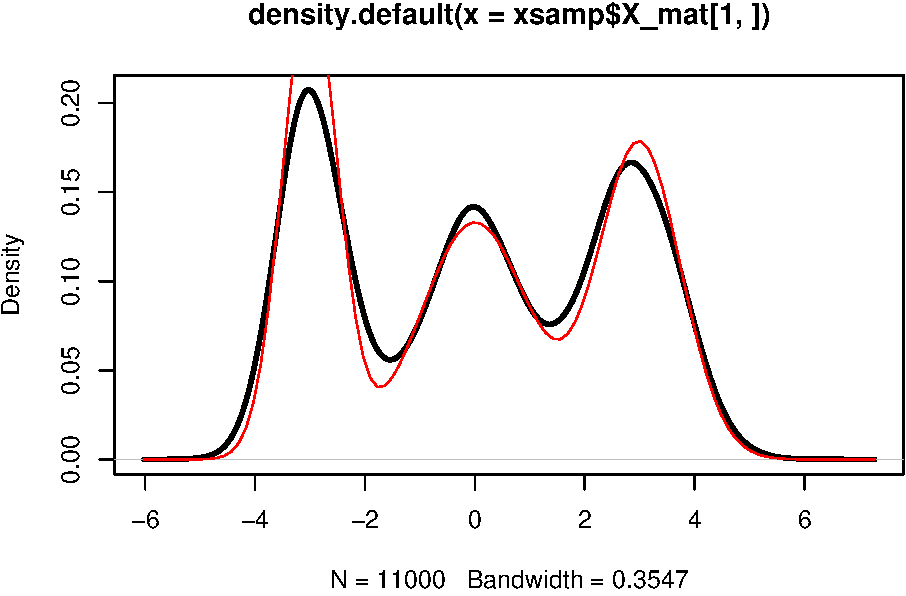
\includegraphics{replication_code_files/figure-latex/unnamed-chunk-6-1.pdf}

\hypertarget{usage-of-package-partemper}{%
\section{\texorpdfstring{Usage of package
\textbf{parTempeR}}{Usage of package parTempeR}}\label{usage-of-package-partemper}}


\end{document}
